% =============================================================
% IEEE iSPEC 2026 Conference Paper  -- VERSION 4
% Rules: IEEEtran, two-column, strict 6 pages
% =============================================================
\documentclass[conference]{IEEEtran}
\IEEEoverridecommandlockouts
\usepackage{cite}
\usepackage{amsmath,amssymb,amsfonts}
\usepackage{algorithmic}
\usepackage{graphicx}
\usepackage{textcomp}
\usepackage{xcolor}
\usepackage{booktabs}
\usepackage{multirow}
\usepackage{url}

\def\BibTeX{{\rm B\kern-.05em{\sc i\kern-.025em b}\kern-.08em
    T\kern-.1667em\lower.7ex\hbox{E}\kern-.125emX}}

\begin{document}

\title{Two-Stage Deep Learning for PV Cell Localization and Defect Triage from Electroluminescence Images%
%\thanks{This work was carried out at [University Name].}
}

% ================================================================
%  AUTHORS
% ================================================================
%\author{%
%\IEEEauthorblockN{1\textsuperscript{st} \textbf{[Author 1 Name]}}
%\IEEEauthorblockA{\textit{\textbf{[Department]}} \\
%\textit{Indian Institute of Technology Mandi}\\
%5Mandi, Himachal Pradesh, India \\
%\textbf{[email@iitmandi.ac.in]}}
%\and
%\IEEEauthorblockN{2\textsuperscript{nd} \textbf{[Author 2 Name]}}
%\IEEEauthorblockA{\textit{\textbf{[Department]}} \\
%\textit{Indian Institute of Technology Mandi}\\
%Mandi, Himachal Pradesh, India \\
%\textbf{[email@iitmandi.ac.in]}}
%}

\maketitle

\begin{abstract}
Automated visual inspection of photovoltaic (PV) modules is critical for scalable quality control, yet most published pipelines assume pre-cropped single-cell inputs and do not address the module-to-cell extraction problem. We present a two-stage deep learning framework consisting of module-to-cell localization and independent cell-level binary triage, evaluated on 4{,}392 module images and 9{,}392 cell crops. Stage~1 adopts YOLOv8-OBB (oriented bounding boxes) for cell extraction after a comparative evaluation of classical OpenCV-based approaches. All five YOLOv8-OBB model scales achieve approximately 0.995 mAP@0.5, with the nano variant reaching 222 FPS. Stage~2 benchmarks seven architectures are ConvNeXt-Tiny, DenseNet-121, MobileNet-V3-Large, ResNet-101, EfficientNet-B4, Swin-S, and ViT-B/16 via Optuna hyperparameter search for binary EL defect triage (OK vs.\ B-grade) on an independent dataset. The two stages are evaluated independently on non-overlapping datasets: a module-level dataset for cell localization and a separate cell-level dataset for binary quality triage. ConvNeXt-Tiny achieves the strongest observed accuracy (97.2\,\%, AUC\,=\,98.6\,\%); DenseNet-121 leads on AUC/PR-AUC (98.9\,\%/99.3\,\%); MobileNet-V3-Large offers the best efficiency at 3.0M parameters.
\end{abstract}

\begin{IEEEkeywords}
Photovoltaic inspection, Electroluminescence, Oriented bounding boxes, Binary defect classification, Deep learning
\end{IEEEkeywords}

%% ============================================================
\section{Introduction}

Global PV capacity is projected to exceed 10~TW by~2030~\cite{iea2023}, placing unprecedented demands on automated quality assurance. Electroluminescence (EL) imaging excites minority carriers with a forward-bias current and records the resulting near-infrared luminescence on a silicon CCD; regions with elevated recombination (cracks, inactive areas, corrosion, delamination) appear as localised dark patches. This modality reveals sub-surface defects invisible to conventional reflected-light or thermal imaging and has become the dominant non-destructive characterisation technique in both manufacturing-line quality control and field fleet inspection.

Automated EL defect analysis has been extensively studied at the \textit{single-cell} level. The canonical ELPV dataset~\cite{deitsch2019} provides 2{,}624 labelled cell-crop images; ResNet and EfficientNet backbones~\cite{he2016,tan2019} achieve binary accuracy exceeding 90\,\% on it. In realistic deployment, however, raw \textit{module-level} images arrive with arbitrary camera orientation, partial occlusion, and perspective distortion. A practical inspection system must first localise and extract individual cells before any per-cell classifier can be applied---yet few robust, format-agnostic plug-in extraction stages have been demonstrated in the published literature.

Three unresolved gaps motivate this work: (1)~classical module-to-cell extraction methods fail to generalise across module formats, EL contrast levels, and camera orientations; (2)~existing binary-triage benchmarks compare only one or two architectures without principled hyperparameter search; (3)~binary OK/B-grade triage is the essential precursor gate for fine-grained pixel-level defect segmentation---incorrect triage propagates errors to all downstream analysis. In this context, OK indicates that a cell is free from any defects, whereas B-grade denotes the presence of at least one defect, such as a crack, inactive region, or gridline failure.

\textbf{Contributions:}
\begin{enumerate}
  \item A systematic evaluation of classical module-to-cell extraction strategies, identifying four major deployment-level failure modes: hyperparameter brittleness, module-format sensitivity, EL-contrast variability, and perspective intolerance.
  \item A format-agnostic YOLOv8-OBB-based cell localization and rectification stage capable of processing full-module, partial-module, and rotated EL images without format-specific geometric tuning, achieving mAP@0.5 $\geq$ 0.9949 and up to 222 FPS.
  \item A comparative benchmark of seven ImageNet-pretrained CNN and Transformer backbones for binary OK/B-grade EL triage under a common Optuna-based hyperparameter-search protocol, including per-class performance, MCC, AUC, PR-AUC, and model-efficiency analysis.
  \item A deployment-oriented analysis of localization accuracy, defective-cell false negatives, model size, and computational efficiency, highlighting ConvNeXt-Tiny, DenseNet-121, and MobileNet-V3-Large as complementary choices for accuracy-, safety-, and resource-constrained inspection scenarios.
\end{enumerate}

%% ============================================================
\section{Related Work}
\label{sec:related}

\textbf{EL datasets.} EL datasets and inspection pipelines. The ELPV dataset~\cite{deitsch2019} containing 2{,}624 pre-cropped grayscale cell images of 300 × 300 pixels, has become a widely used benchmark for cell-level EL defect classification. Consequently, much of the existing literature evaluates classification after individual cells have already been extracted. In practical manufacturing or field inspection, however, the input is typically a full or partial module-level EL image, requiring reliable localization and rectification of individual cells before defect classification. Although several studies have investigated automated PV defect detection~\cite{zhao2022, su2021, li2023, chen2024, wang2023}, robust module-to-cell localization across heterogeneous module formats, image orientations, contrast conditions, and partial-module views remains comparatively less explored.

\textbf{Classical cell extraction.} Hough-transform line detection~\cite{duda1972}, morphological grid extraction~\cite{soille2003}, and projection-profile peak finding~\cite{wong1982} are the three main classical families. All rely on manually set thresholds (Hough rho/theta resolution, DBSCAN~$\epsilon$, CLAHE clip limits) that must be retuned per dataset and fail under even moderate camera tilt, non-uniform EL illumination, or partial module occlusion---as our classical-extraction experiments confirm.

\textbf{Object detection.} YOLO-family single-stage detectors~\cite{redmon2016,jocher2023} dominate real-time industrial visual inspection. YOLOv8-OBB~\cite{jocher2023} extends the axis-aligned formulation with an explicit rotation-angle regression head, allowing tight-fitting detection of arbitrarily oriented rectangular objects without a preprocessing rectification step.

\textbf{Classification backbones.} ResNet~\cite{he2016} and EfficientNet~\cite{tan2019} are the most commonly reported backbones for EL defect classification. ConvNeXt~\cite{liu2022} modernises the pure-CNN architecture with large-kernel depthwise convolutions and layer-norm, outperforming ResNets on fine-grained visual tasks. Swin Transformer~\cite{liu2021} introduces a hierarchical shifted-window self-attention that rivals CNNs on medium-scale datasets. Neither has been systematically compared against CNNs on EL imagery under Bayesian hyperparameter search~\cite{akiba2019}.

\textbf{Class imbalance.} EL datasets are naturally imbalanced: defective cells (B-grade) outnumber functional ones in aged or stressed modules. Standard accuracy is misleading under imbalance; AUC and Matthews Correlation Coefficient (MCC)~\cite{deitsch2019} are more informative threshold-independent metrics. We adopt AUC as the Optuna objective and report MCC alongside per-class precision/recall.

%% ============================================================
\section{Dataset}
\label{sec:dataset}

\subsection{Stage 1: Module-Level Dataset for Cell Extraction}
Stage~1 contains 4{,}392 JPEG EL images from ARTS, SDLE, BMRK ~\cite{pratt2023benchmark}, comprising both full modules (predominantly 144-cell formats) and partial module crops (typically containing 1--2 complete cells alongside fragments of neighbouring cells). These are annotated with oriented bounding boxes for cell localization using Roboflow by a domain expert and cross-verified. The split assigns 3{,}909 images to training (89\,\%), 322 to validation (7\,\%), and 161 to testing (4\,\%). Preprocessing includes auto-orientation, conversion to grayscale, adaptive contrast equalization, and resizing (stretched to $640\times640$~px). During training, augmentation (flip, $\pm11^\circ$ rotation, $\pm8^\circ$ shear, brightness/noise jitter) generates 3 variants per example to improve generalisation. The Stage~1 dataset is used exclusively for cell-localization experiments and is not used to train or evaluate the Stage~2 defect classifier.

\subsection{Stage 2: Independent Cell-Level Dataset for Triage}
Stage~2 uses an independent cell-level EL dataset obtained from a separate source. The Stage~1 module images and their extracted cell crops are \textit{not} included in the Stage~2 partitions. Labels are binarised into OK and B-grade categories, with B-grade treated as the positive class. In this study, B-grade denotes cells that fail the adopted EL quality criterion because of one or more visible defect signatures, such as cracks, inactive regions, gridline breaks, or ribbon failures. The dataset comprises 9{,}392 cells, partitioned with a module-level group split to prevent spatial correlation across folds. Table~\ref{tab:datasplit} reports statistics. The test set is 67.4\,\% OK / 32.6\,\% B-grade.

\begin{table}[t]
  \caption{Stage~2 independent dataset split statistics}
  \label{tab:datasplit}
  \begin{center}
  \renewcommand{\arraystretch}{1.05}\small
  \begin{tabular}{lrrr}
    \toprule
    \textbf{Split} & \textbf{Total} & \textbf{OK} & \textbf{B-grade}\\
    \midrule
    Train & 6{,}575 & 4{,}428 & 2{,}147\\
    Val   & 1{,}408 &   954   &   454\\
    Test  & 1{,}409 &   949   &   460\\
    \bottomrule
  \end{tabular}
  \end{center}
\end{table}

\subsection{Preprocessing}
Single-channel 8-bit grayscale $\to$ median blur ($3\times3$, noise suppression) $\to$ CLAHE (clipLimit\,=\,2.0, tileGridSize\,=\,$8\times8$, EL normalisation) $\to$ \texttt{cv2.warpPerspective} (canonical upright crops) $\to$ zero-mean unit-variance normalisation.

%% ============================================================
\section{Methodology}
\label{sec:method}

\subsection{Stage 1: Cell Extraction}
\label{sec:stage1}

\subsubsection{Evaluation of Classical Cell-Extraction Strategies}

Multiple classical cell-extraction approaches were evaluated on both partial/single-cell and full-module EL images, including projection profiles, morphological processing, contour extraction, Hough-line detection, polynomial fitting, and Hough–DBSCAN clustering. Rather than relying on notebook-specific implementations, the comparison focuses on the dominant failure modes observed across representative classical approaches.

\begin{table}[t]
  \caption{Classical extraction exploration failure summary}
  \label{tab:classical_all}
  \begin{center}
  \renewcommand{\arraystretch}{1.0}\scriptsize
  \begin{tabular}{p{0.55cm}p{0.35cm}p{1.65cm}p{3.55cm}}
    \toprule
    \textbf{NB} & \textbf{Trk} & \textbf{Technique} & \textbf{Key Failure}\\
    \midrule
    pp1  & C & CLAHE+profiles   & Exploratory; no extraction\\
    pp2  & C & Morph.+warp      & Single image; not generalised\\
    pp3  & C & Inv.+contour     & Conflates cell/defect regions\\
    pp4  & C & Batch extractor  & \textbf{5--10\,\% skip rate}\\
    pp5  & C & ---              & YOLO pivot notebook\\
    pp6  & C & Gaussian+Canny   & Fragmented contours\\
    pp7  & C & NL-Means+Hough   & Image-specific threshold\\
    pp8  & C & Multi-cell Hough & Requires a priori line count\\
    pp9  & C & Otsu+Canny       & Format-specific count limit\\
    pp10 & C & Otsu+poly.\ fit  & Fails on multi-cell images\\
    pp11 & C & Hough+DBSCAN     & Dataset-specific $\epsilon$\\
    \midrule
    fmv1 & F & HoughLinesP      & Near-duplicate lines; unusable\\
    fmv2 & F & Proj.\ peaks     & \textbf{144 cells OK}; format-specific\\
    fmv3 & F & Batch fmv2       & 208 vs.\ 182 cells, same format\\
    fmv4 & F & DBSCAN merging   & Needs manual count verification\\
    \bottomrule
    \multicolumn{4}{l}{\scriptsize C\,=\,CellExtract; F\,=\,FullModule track.}
  \end{tabular}
  \end{center}
\end{table}

Four recurring failure modes were identified across the evaluated classical methods: (1) hyperparameter brittleness, where CLAHE settings, Hough thresholds, and DBSCAN parameters required image-specific tuning; (2) module-format sensitivity, where projection-based counting produced inconsistent cell estimates across nominally similar modules; (3) contrast variability, where low-EL regions caused busbar or cell-boundary responses to fall below detection thresholds; and (4) perspective intolerance, where axis-aligned morphological and line-detection assumptions degraded under moderate module tilt.

\subsubsection{YOLOv8-OBB: Unified Final Approach}
\label{sec:yolo}

\textbf{Why not axis-aligned YOLO?} Standard axis-aligned YOLO detectors must \textit{fully enclose} a rotated object with an upright rectangle. For a $10^\circ$-tilted $144\times144$~px PV cell, the enclosing axis-aligned bounding box expands to $\approx$$\!167\times167$~px---a 34\,\% area increase---wasting roughly 25\,\% of the box area on background busbar and inter-cell gaps. This background contamination degrades the quality of the Stage~2 classification crop and, more critically, causes heavy IoU overlap between adjacent enclosing boxes: the NMS suppression threshold then erroneously removes valid cell detections, leading to systematic missed extractions in tilted modules. YOLOv8-OBB directly regresses $\theta$ alongside $(c_x, c_y, w, h)$, keeping the fitted box tight to the cell boundary regardless of orientation.

YOLOv8-OBB (Ultralytics~8.3.235~\cite{jocher2023}) was adopted as the sole Stage~1 detector. Each detection outputs a five-parameter oriented bounding box:
\begin{equation}
  \mathbf{d} = (c_x,\; c_y,\; w,\; h,\; \theta),
  \label{eq:obb}
\end{equation}
where $c_x, c_y \in \mathbb{R}$ are the centre pixel coordinates; $w, h \in \mathbb{R}^{+}$ are the width and height along the rotated axes; and $\theta \in [-90^\circ, 90^\circ)$ is the clockwise rotation angle of the box's major axis relative to the horizontal.

Post-processing converts each OBB to a rectified cell crop:
\begin{equation}
  (c_x, c_y, w, h, \theta)
  \xrightarrow{\;\text{corners}\;}
  M_{\text{persp}}
  \xrightarrow{\;\texttt{warpPersp.}\;}
  \hat{I}_{\text{cell}},
  \label{eq:postproc}
\end{equation}
where the \textit{corners} step maps OBB parameters to four corner coordinates $\{p_i\}_{i=1}^{4}$; $M_{\text{persp}} \in \mathbb{R}^{3\times3}$ is the perspective transformation matrix from \texttt{cv2.getPerspectiveTransform}; and $\hat{I}_{\text{cell}} \in \mathbb{R}^{H_0 \times W_0}$ is the canonical upright crop at fixed resolution $H_0 \times W_0$.

\subsection{Stage 2: Binary Quality Triage}
\label{sec:stage2}

\subsubsection{Benchmark Design}
Seven ImageNet-pretrained backbone families were fine-tuned end-to-end: ConvNeXt-Tiny, DenseNet-121, MobileNet-V3-Large, ResNet-101, EfficientNet-B4, Swin-Small, and ViT-B/16. Each model uses the same head architecture: global average pooling $\to$ dropout $\to$ a single linear layer producing one logit. The classifier was trained using class-weighted binary cross-entropy with logits (to address the OK:B-grade training-set imbalance), and a sigmoid activation was applied only during inference. All models are trained with early stopping (patience 10 epochs on validation AUC) to prevent overfitting on the 6{,}575-sample training set.

Data augmentation during training (applied on-the-fly): random horizontal/vertical flip, random rotation $\pm15^\circ$, random brightness/contrast jitter ($\pm$15\,\%), Gaussian blur ($\sigma \in [0.5, 1.5]$), and random erasing (probability 0.2, area ratio 0.02--0.15). All augmentations are implemented via \ \texttt{torchvision.transforms} and applied only during training.

\subsubsection{Hyperparameter Search via Optuna}
Each backbone receives an identical budget of 30 Optuna trials using Tree-structured Parzen Estimator (TPE) sampling~\cite{akiba2019}, each capped at 15 epochs, followed by a final 40-epoch training run for the best configuration. The search space is defined in Table~\ref{tab:optuna_space}. The objective metric is validation AUC, chosen for its threshold-invariance under the class imbalance. Fig.~\ref{fig:optuna_importance} shows the hyperparameter-importance scores for ConvNeXt-Tiny, derived using fANOVA on the completed Optuna trials. For this backbone, weight decay, freeze strategy, and batch size were the most influential hyperparameters affecting validation AUC.

\begin{table}[t]
  \caption{Optuna search space (Stage~2)}
  \label{tab:optuna_space}
  \begin{center}
  \renewcommand{\arraystretch}{1.05}\small
  \begin{tabular}{p{2.1cm}p{5.1cm}}
    \toprule
    \textbf{Hyperparameter} & \textbf{Search Space}\\
    \midrule
    Learning rate   & LogUniform$[10^{-5},\;10^{-2}]$\\
    Weight decay    & LogUniform$[10^{-6},\;10^{-2}]$\\
    Optimizer       & \{Adam, AdamW, SGD+mom.\}\\
    LR scheduler    & \{cosine, step, plateau\}\\
    Dropout         & Uniform$[0.01,\;0.5]$\\
    Batch size      & \{16, 32, 64\}\\
    Freeze strategy & \{none, partial, full\}\\
    Objective       & Validation AUC\\
    \bottomrule
  \end{tabular}
  \end{center}
\end{table}

\begin{figure}[t]
  \centering
  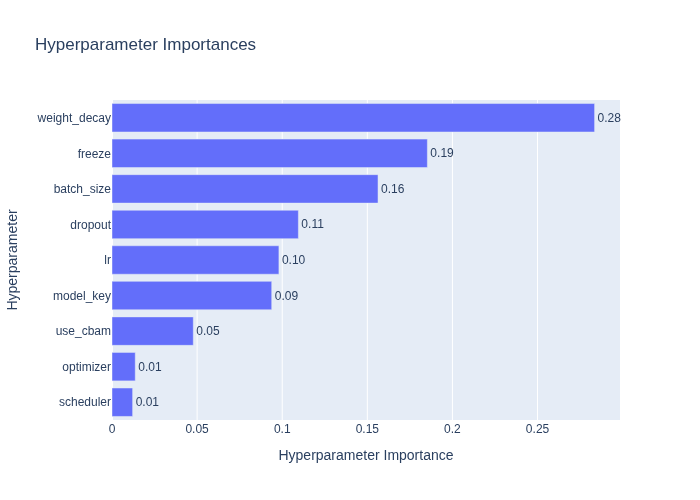
\includegraphics[width=\columnwidth]{fig_optuna_importance.png}
  \caption{Optuna hyperparameter importance (ConvNeXt-Tiny, Stage~2). Weight decay, freeze strategy, and batch size are the dominant factors, consistent across all seven backbones. Note: \texttt{model\_key} and \texttt{use\_cbam} appear in the fANOVA analysis from a broader ablation study encompassing all architectures and attention modules.}
  \label{fig:optuna_importance}
\end{figure}

%% ============================================================
\section{Experimental Setup}
\label{sec:setup}

\textbf{Hardware:} NVIDIA RTX PRO 4500 Blackwell GPU; AMD Ryzen Threadripper 7960X (48 threads); 192~GB RAM; Ubuntu~24.04.2 LTS (Linux~6.17, 64-bit).

\textbf{Software:} Python~3.x, PyTorch, Ultralytics~8.3.235, \texttt{timm}, Optuna, OpenCV~4.12.0.88, NumPy~1.26.4, scikit-learn, Matplotlib~3.8.4.

\textbf{Reproducibility:} All reported results are based on a single fixed random seed. Consequently, small performance differences between closely ranked models should be interpreted cautiously, as run-to-run variance has not yet been quantified.

%% ============================================================
\section{Results}
\label{sec:results}

\subsection{Stage 1: Cell Extraction}

Table~\ref{tab:stage1_results} benchmarks all five YOLOv8-OBB scales on the 161-image test set. All variants achieve mAP@0.5\,=\,0.9950 with perfect recall (1.0000), indicating that the localization task is already near saturation at the lightest model scale. YOLOv8n-OBB (3.1M parameters, 4.5~ms/image) is the recommended deployment variant. The strongest classical pipeline was not included in the mAP comparison because it did not produce annotation-compatible oriented bounding boxes and still required manual verification of extracted cell counts.

\begin{table}[t]
  \caption{Stage~1 YOLOv8-OBB benchmark (test set, 161 images)}
  \label{tab:stage1_results}
  \begin{center}
  \renewcommand{\arraystretch}{1.05}\small
  \begin{tabular}{lrrrr}
    \toprule
    \textbf{Model} & \textbf{Params} & \textbf{FPS} & \textbf{mAP@.5} & \textbf{mAP@.5:.95}\\
    \midrule
    YOLOv8n-OBB & 3.1M  & \textbf{222} & 0.9950 & 0.9909\\
    YOLOv8s-OBB & 11.4M & 216          & 0.9950 & 0.9932\\
    YOLOv8m-OBB & 26.4M & 148          & 0.9950 & \textbf{0.9947}\\
    YOLOv8l-OBB & 44.5M & 118          & 0.9949 & 0.9919\\
    YOLOv8x-OBB & 69.5M & 86           & 0.9950 & 0.9921\\
    \midrule
  \end{tabular}
  \end{center}
\end{table}

Fig.~\ref{fig:yolo_detections} shows YOLOv8n-OBB predictions on EL module images from the validation set.

\begin{figure}[t]
  \centering
  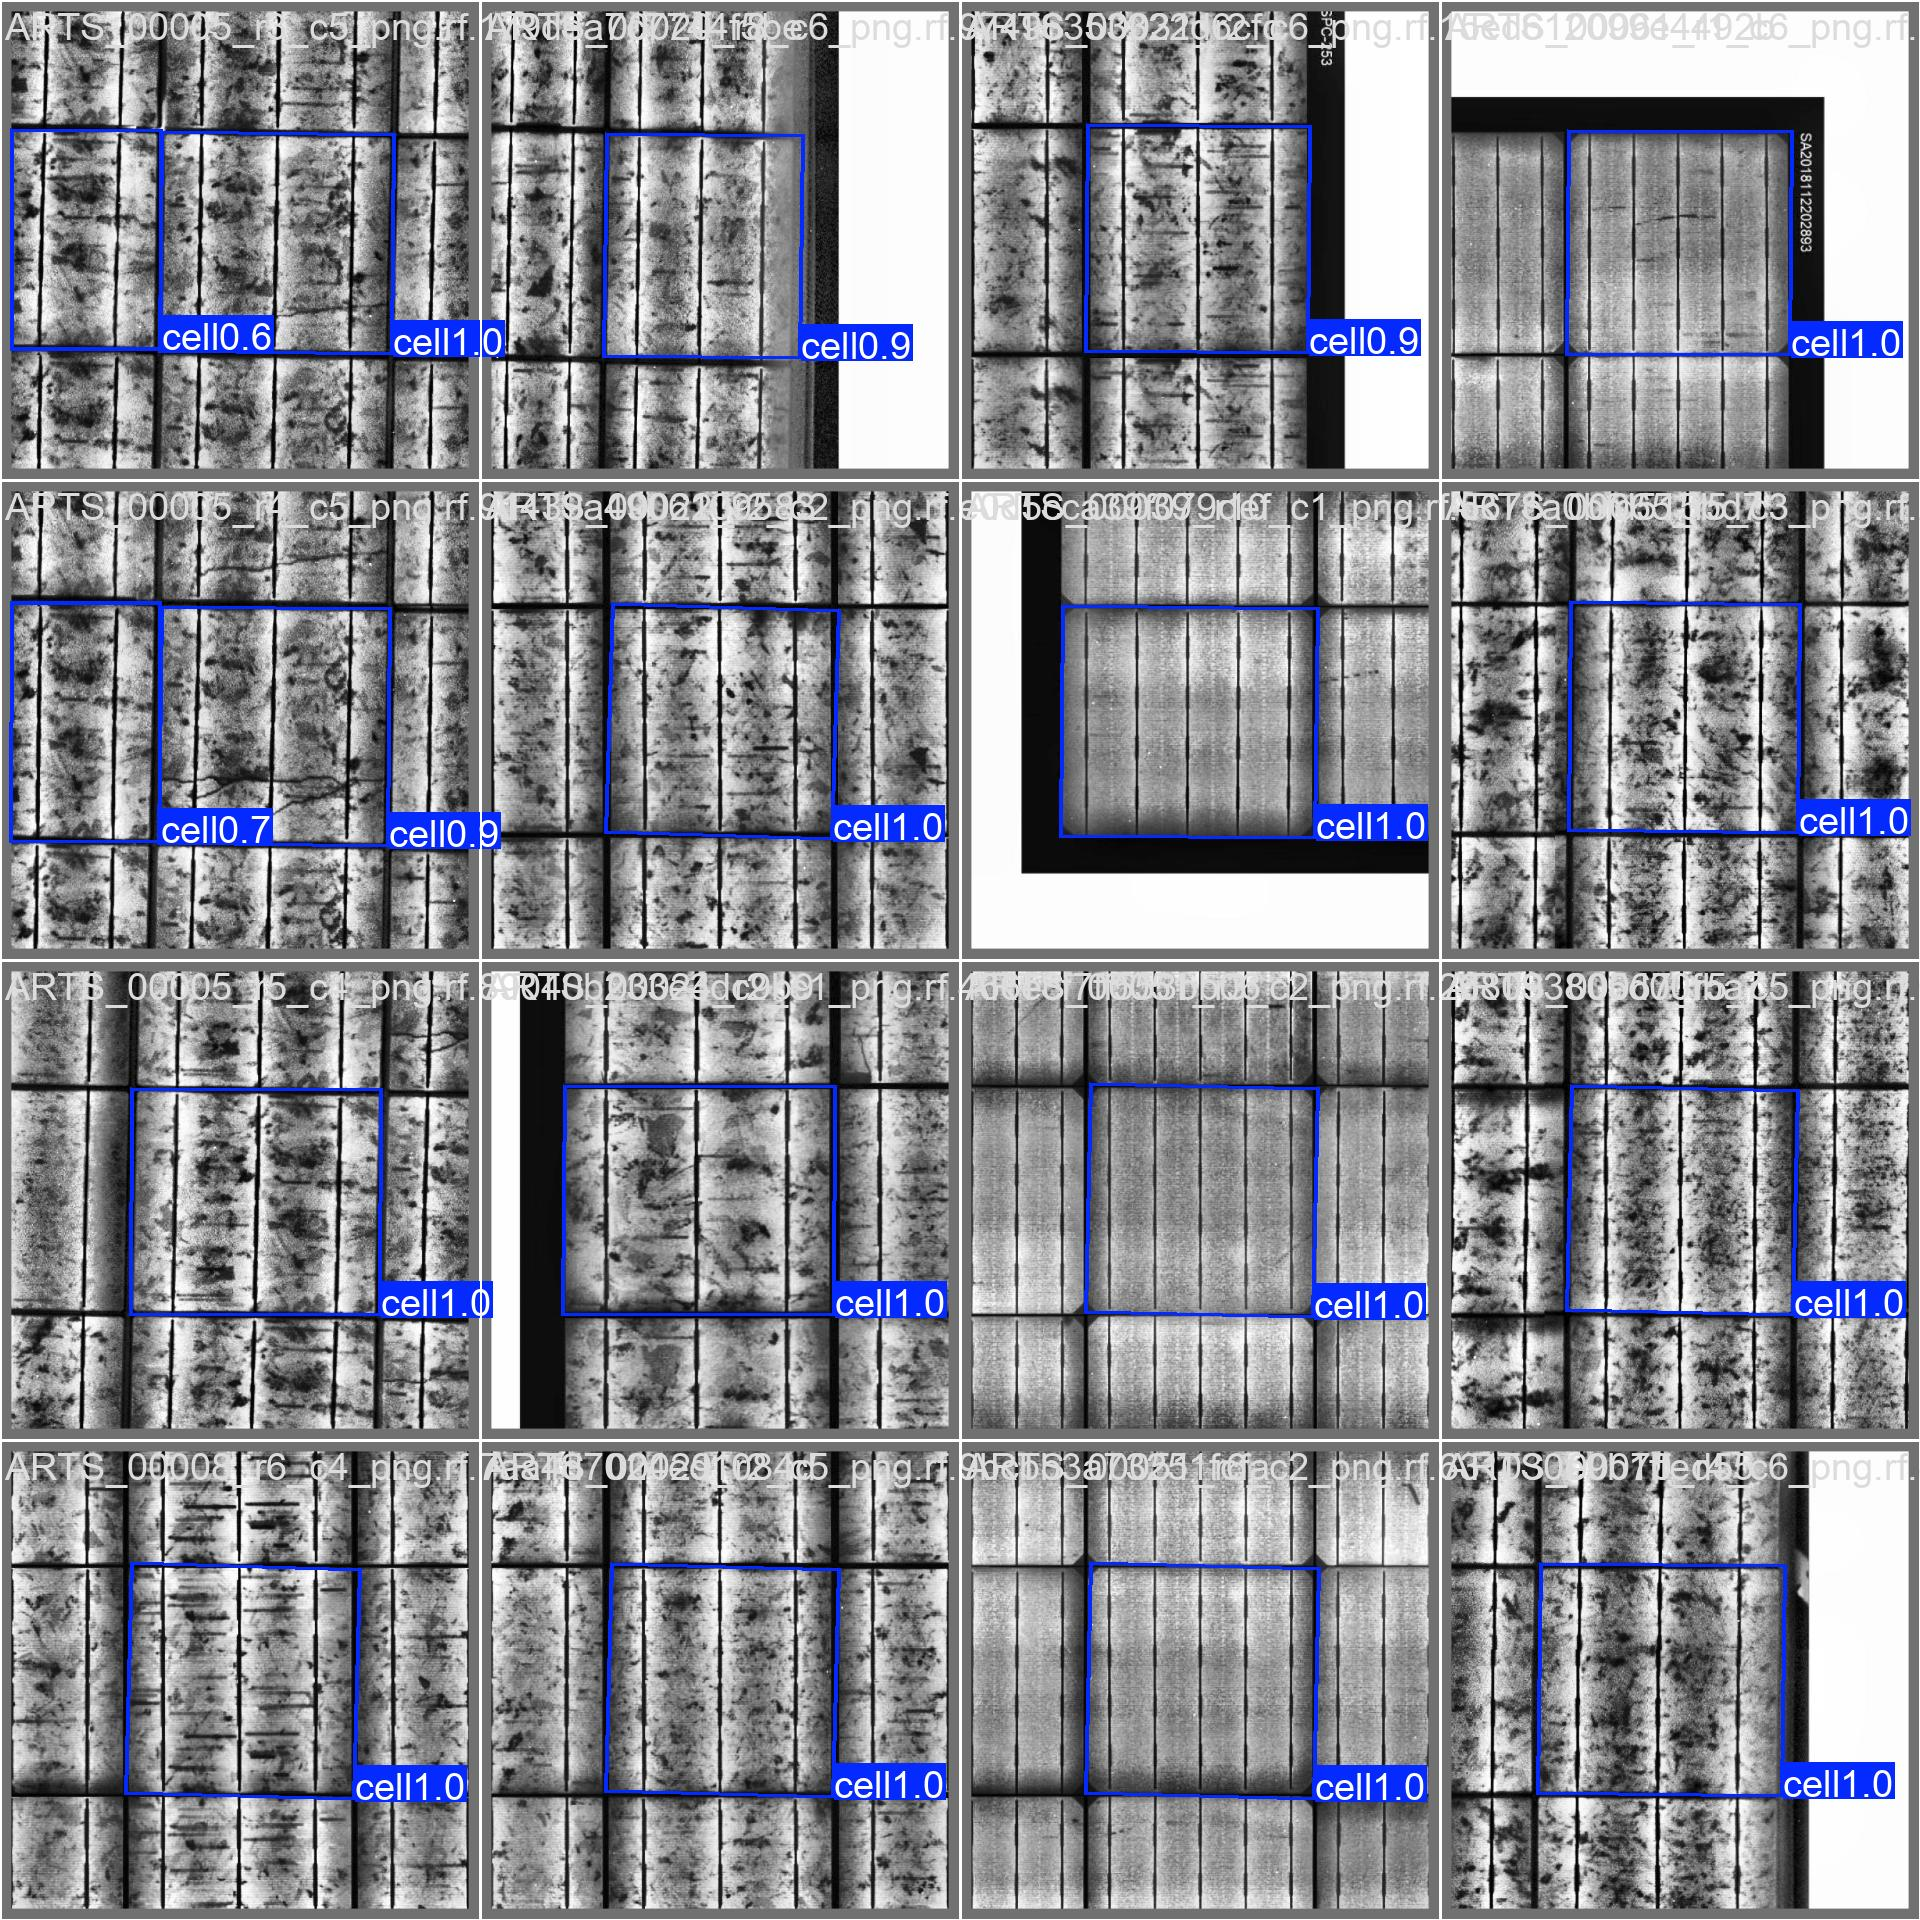
\includegraphics[width=\columnwidth,height=7cm,keepaspectratio=false]{fig_yolo_detections.jpg}
  \caption{Representative YOLOv8n-OBB predictions on module-level EL images. The oriented bounding boxes remain aligned with individual cell boundaries under module rotation, enabling subsequent perspective rectification into canonical upright crops for Stage-2 classification.}
  \label{fig:yolo_detections}
\end{figure}

\subsection{Stage 2: Binary Quality Triage}

Tables~\ref{tab:stage2_results}--\ref{tab:stage2_perclass} present the seven-architecture Optuna benchmark on 1{,}409 test images, comprising 949 OK, 460 B-grade. ConvNeXt-Tiny achieves the highest accuracy (97.2\,\%) and MCC (93.7\,\%); DenseNet-121 achieves the highest AUC (98.9\,\%) and PR-AUC (99.3\,\%). MobileNet-V3-Large achieves the same test accuracy as ResNet-101 (96\%) while using approximately $14\times$ fewer parameters (3.0M vs. 42.5M), making it the most attractive model-size/performance trade-off among the evaluated architectures. Transformer-based Swin-S and ViT-B/16 rank last on all primary metrics, suggesting that Swin-S and ViT-B/16 underperformed the evaluated CNNs on this dataset under our training protocol. The observed accuracies are also higher than early SVM ($\approx$73\,\%) and CNN ($\approx$82\,\%) results reported on ELPV~\cite{deitsch2019}, although direct numerical comparison should be interpreted cautiously because our dataset composition and splitting protocol differ.

\begin{table}[t]
  \caption{Stage~2 binary triage: 7-architecture Optuna benchmark (test set; best trial per backbone)}
  \label{tab:stage2_results}
  \begin{center}
  \renewcommand{\arraystretch}{1.05}\small
  \setlength{\tabcolsep}{3.0pt}
  \begin{tabular}{p{1.75cm}rp{0.6cm}p{0.65cm}p{0.65cm}p{0.72cm}p{0.65cm}}
    \toprule
    \textbf{Model} & \textbf{Par.} & \textbf{Acc.} & \textbf{F1-M} & \textbf{AUC} & \textbf{PR-AUC} & \textbf{MCC}\\
    \midrule
    \textbf{ConvNeXt-T} & 27.8M & \textbf{.972} & \textbf{.968} & .986 & .989 & \textbf{.937}\\
    DenseNet-121        &  7.0M & .969           & .964          & \textbf{.989} & \textbf{.993} & .929\\
    MobileNet-V3L       &  3.0M & .960           & .954          & .970 & .973 & .909\\
    ResNet-101          & 42.5M & .960           & .953          & .980 & .988 & .908\\
    EffNet-B4           & 17.6M & .952           & .946          & .984 & .984 & .891\\
    Swin-S              & 48.8M & .949           & .940          & .976 & .986 & .884\\
    ViT-B/16            & 85.8M & .946           & .937          & .977 & .985 & .877\\
    \bottomrule
    \multicolumn{7}{l}{\footnotesize Par.\,=\,Parameters (M); F1-M\,=\,F1-Macro; MCC\,=\,Matthews Corr.\ Coeff.}
  \end{tabular}
  \end{center}
\end{table}

\begin{table}[t]
  \caption{Stage~2 per-class precision/recall (test set; OK\,=\,949, B-grade\,=\,460)}
  \label{tab:stage2_perclass}
  \begin{center}
  \renewcommand{\arraystretch}{1.05}\small
  \setlength{\tabcolsep}{3.0pt}
  \begin{tabular}{p{1.75cm}p{0.6cm}p{0.6cm}p{0.6cm}p{0.6cm}rr}
    \toprule
    \textbf{Model} & \textbf{OK-P} & \textbf{OK-R} & \textbf{BG-P} & \textbf{BG-R} & \textbf{FP} & \textbf{FN}\\
        \midrule
    \textbf{ConvNeXt-T} & .970 & .989 & .977 & .937 & 10 & 29\\
    DenseNet-121        & .974 & .980 & .958 & .946 & 19 & 25\\
    MobileNet-V3L       & .953 & .989 & .976 & .900 & 10 & 46\\
    ResNet-101          & .953 & .988 & .974 & .900 & 11 & 46\\
    EffNet-B4           & .958 & .972 & .940 & .913 & 27 & 40\\
    Swin-S              & .936 & .992 & .980 & .861 &  8 & 64\\
    ViT-B/16            & .936 & .987 & .971 & .861 & 12 & 64\\
    \bottomrule
    \multicolumn{7}{l}{\footnotesize FP\,=\,OK misclassified as BG; FN\,=\,BG misclassified as OK.}
  \end{tabular}
  \end{center}
\end{table}

Fig.~\ref{fig:stage2_roc} shows ROC curves; Fig.~\ref{fig:stage2_paramsf1} shows the parameters-vs.-F1 efficiency trade-off.

\begin{figure}[t]
  \centering
  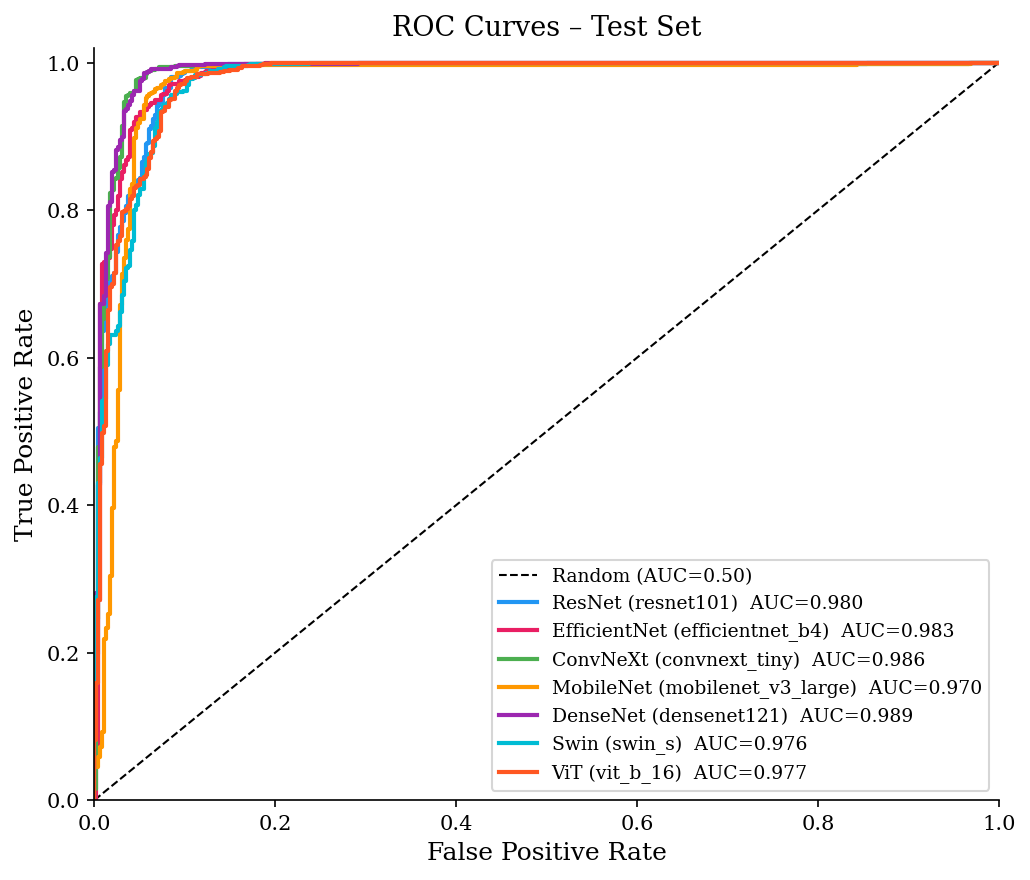
\includegraphics[width=\columnwidth,height=6cm]{fig_stage2_roc.png}
  \caption{ROC curves (test set) for all seven Stage~2 architectures. DenseNet-121 (AUC\,=\,0.989) and ConvNeXt-Tiny (AUC\,=\,0.986) are the leading models; Transformer-based Swin-S and ViT-B/16 lag all CNN-based variants.}
  \label{fig:stage2_roc}
\end{figure}

\begin{figure}[t]
  \centering
  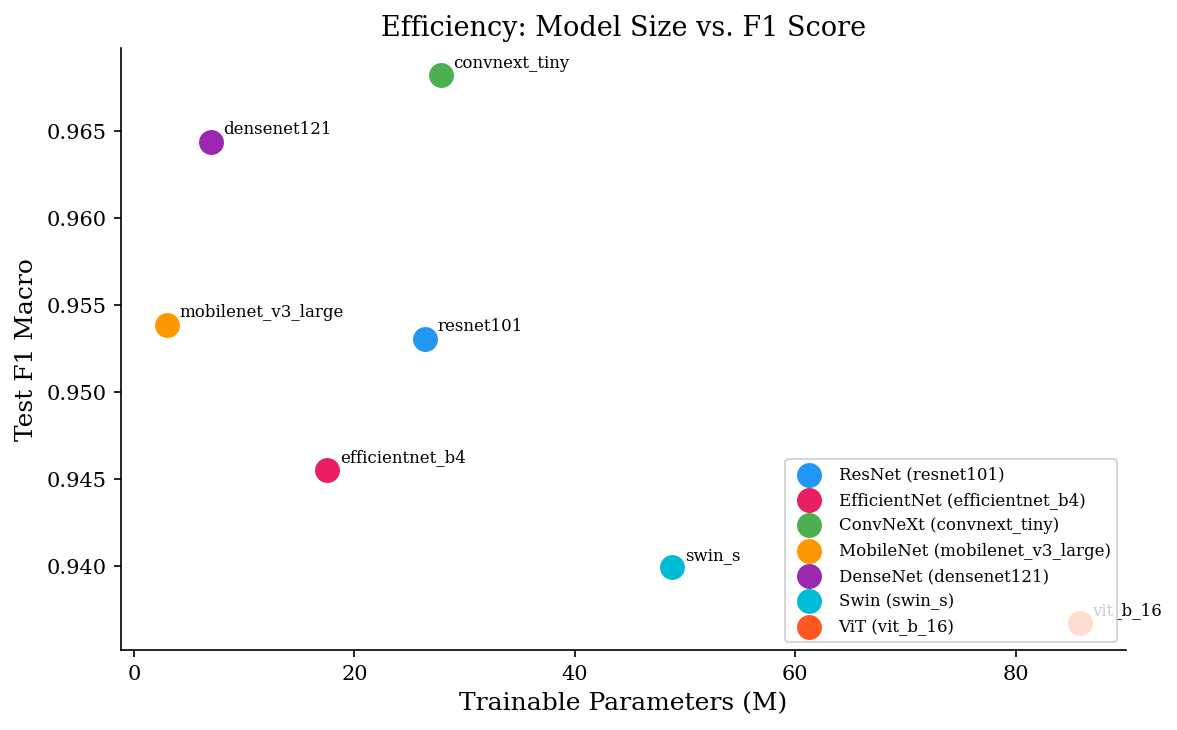
\includegraphics[width=\columnwidth, height=5.5cm]{fig_stage2_paramsf1.png}
  \caption{Model size versus test F1-macro for the seven Stage-2 architectures. MobileNet-V3-Large achieves a favourable efficiency point at 3.0M parameters and F1-macro = 0.954, while larger models do not consistently yield higher classification performance.}
  \label{fig:stage2_paramsf1}
\end{figure}

%% ============================================================
\section{Discussion}
\label{sec:discussion}

\subsection{Stage 1: Task Saturation and Leakage Verification}

All five YOLOv8-OBB variants achieve mAP@0.5\,=\,0.9950 with perfect recall (1.0000). This saturation is consistent with the visual regularity of PV cell grids: once the detector learns the periodic busbar-and-boundary signature from a sufficiently diverse set of module images, additional model capacity yields diminishing returns in detection quality. The mAP@0.5:0.95 metric, which penalises imprecise localisation, shows a more meaningful spread (0.9909 for nano, 0.9947 for medium), indicating that larger models produce marginally tighter OBBs at the cost of throughput. Dataset partitioning was performed at the physical-module level rather than at the individual-cell or image-crop level. All images and cell instances originating from the same physical PV module were assigned exclusively to a single partition (training, validation, or test), preventing identical or spatially correlated cells from appearing across splits and thereby reducing the risk of data leakage.

The nano variant's 4.5~ms total per-image latency (1.4~ms preprocess, 1.2~ms inference, 2.0~ms postprocess on the RTX PRO 4500) makes real-time manufacturing-line integration feasible. A 72-cell module (a common industrial configuration) yields 72 crops in $<$5~ms from the OBB stage, all fed to Stage~2 in a single batched inference pass.

\subsection{Stage 2: CNN Inductive Bias on Small Data}

Under the evaluated dataset size and training protocol, the CNN-based models consistently outperformed the two Transformer-based models, Swin-S and ViT-B/16, across the primary metrics. One plausible explanation is that the locality and translation-equivariance priors of CNNs provide useful regularisation for this relatively small EL dataset, whereas attention-based architectures may require different optimisation settings or greater data diversity to realise their full advantage. ConvNeXt-Tiny and DenseNet-121 achieved closely matched performance; however, the current single-run evaluation does not support a claim of statistically significant superiority between them. ConvNeXt-Tiny provided the strongest observed accuracy--MCC trade-off, while DenseNet-121 achieved the highest single-run AUC and PR-AUC in our experiments.

\textbf{Optimal hyperparameters.} Across all backbones, Optuna consistently selected AdamW as the best optimiser with a cosine or step LR schedule. The best learning rates cluster in the range $[10^{-4}, 4×10^{-4}]$ for CNN-based models and $[2×10^{-5}, 3×10^{-5}]$ for Transformer-based models, consistent with the lower learning rates typically required for fine-tuning attention-heavy architectures. Dropout rates vary widely (0.02--0.50), but have lower Optuna importance scores than LR and weight decay (Fig.~\ref{fig:optuna_importance}).

\textbf{False-negative analysis.} In quality-critical manufacturing, false negatives are particularly important because a B-grade cell misclassified as OK may pass downstream quality gates and contribute to avoidable yield or reliability loss. DenseNet-121 produced the fewest false negatives (25/460), whereas ConvNeXt-Tiny produced 29 false negatives and 10 false positives, resulting in the lowest total error count (39) among the evaluated models. Swin-S achieved the lowest false-positive count (8) but incurred 64 false negatives, illustrating the importance of considering class-specific risk rather than accuracy alone.

\textbf{End-to-end latency.} Stage~1 processes one full module image in $\approx$4.5~ms (222~FPS). Stage-2 inference latency was not directly benchmarked in the present study; therefore, no quantitative latency claim is made for the classification stage. Rigorous benchmarking of single-cell and batched classification inference on the RTX PRO 4500 is reserved for future work. The measured 4.5-ms Stage-1 latency demonstrates that cell localization itself is compatible with real-time operation; however, overall pipeline throughput can only be established after jointly benchmarking OBB detection, crop rectification, and batched Stage-2 classification.

\subsection{Limitations}

\textit{Domain gap:} All training and evaluation use laboratory EL images acquired under controlled forward-bias conditions. Field-acquired EL images (outdoor, drone-mounted) introduce JPEG compression artefacts, solar background illumination, and varying forward-bias current levels, which degrade model performance. Domain adaptation strategies (adversarial alignment, test-time augmentation) are a high-priority follow-on.

\textit Future work will also examine whether lightweight channel/spatial attention modules can improve sensitivity to localized B-grade defect signatures without substantially increasing inference cost.

\textit{Single-seed results:} All experiments report single-run performance with a fixed random seed. Future work will include multi-seed evaluation and statistical comparison of the highest-performing models to quantify run-to-run variance and determine whether the observed differences between ConvNeXt-Tiny and DenseNet-121 are statistically meaningful.

\textit{Annotation cost:} OBB labelling of 4{,}392 EL images required significant manual effort. Semi-supervised or weakly supervised cell detection---using the OBB model to pseudo-label unlabelled modules---is a natural next step to scale annotation.

%% ============================================================
\section{Conclusion and Future Work}
\label{sec:conclusion}

We presented a two-stage framework for automated PV EL inspection comprising module-to-cell localization and independent cell-level binary quality triage. The two stages were evaluated independently on separate datasets, establishing the performance of each component while avoiding cross-stage data leakage. A systematic evaluation of classical OpenCV approaches identified four fundamental failure modes (hyperparameter brittleness, format sensitivity, contrast variability, perspective intolerance) that rendered heuristic methods unreliable across our heterogeneous module dataset. YOLOv8-OBB substantially mitigates these failure modes, with all evaluated scales achieving mAP@0.5 $\geq$ 0.9949 and the nano variant reaching 222 FPS, indicating strong potential for real-time cell localization. A comparative evaluation of seven widely used backbone architectures for binary OK/B-grade triage identifies ConvNeXt-Tiny (Acc.\,97.2\,\%, AUC\,98.6\,\%, FN\,=\,29) as providing the strongest observed accuracy--MCC trade-off, and DenseNet-121 (AUC\,98.9\,\%, PR-AUC\,99.3\,\%, FN\,=\,25) as achieving the highest single-run AUC and lowest false negative count. MobileNet-V3-Large achieves the same accuracy as ResNet-101 with $14\times$ fewer parameters, making it a promising candidate for future edge deployment.

\textbf{Future work:} Future work will focus on end-to-end benchmarking of pipeline latency on edge hardware (NVIDIA Jetson Orin), rigorous multi-seed statistical validation of the model performance differences, and exploring domain adaptation strategies (adversarial alignment, test-time augmentation) to align the lab-EL model to field-acquired EL/IR imagery for reliable fleet inspection. A key next step is a true end-to-end evaluation in which raw module-level EL images are passed through localization, perspective rectification, and cell-level triage on a common independently labelled test set.

\bibliographystyle{IEEEtran}
\bibliography{references}

\end{document}